% Paper exhibits with draft captions. Every number in a caption is read from saved run tables
% (experiments/oversight/make_paper_exhibits.py and the per-study results notes).
% Plain-language rule: every technical term used here is defined in the Key terms table.

\begin{table}[H]
  \centering\small
  \caption{\textbf{Key terms.} The words used in the figures and tables, in plain language.}
  \label{tab:glossary}
  \begin{tabular}{@{}p{0.24\textwidth}p{0.72\textwidth}@{}}
\toprule
Term & Meaning in this paper \\
\midrule
\multicolumn{2}{@{}l}{\emph{The game}} \\
Agent & One of six participants who draw on the shared resource each step (a fisher in \textsc{Fishery}, a forester in \textsc{Forest}, a factory in \textsc{River}). \\
Greedy agent & An agent whose fixed rule asks for a lot; 2 or 4 of the 6 in most runs. \\
Request $p_i$ & How much an agent asks to take this step, as a share of its maximum. \\
Report & What the agent tells the reviewer it wants. An honest report equals the request; an \emph{under-report} (a lie) is smaller. \\
Allowance & What the reviewer lets an agent take this step: its request times the shared cut. \\
Over-taking (cheating) & Taking more than the allowance. Nobody sees it unless the agent is audited. \\
Step, run & One round of requests and harvest; a run is 80 steps. \\
Population (context) & One randomly generated set of six agents and its random seeds. Results average over 64 of them. \\
\addlinespace
\multicolumn{2}{@{}l}{\emph{The reviewer}} \\
Reviewer & The overseer. It predicts what the requests would do to the resource and approves them or cuts them back. \\
Shared cut $\lambda$ & One scaling factor (1, $\tfrac34$, $\tfrac12$, $\tfrac14$ or 0) applied to everyone's request. \\
Model of the resource & The reviewer's equations for how the resource regrows. ``Correct model'' means it knows the true ones. \\
Joint reviewer & Adds up all six requests before predicting. \\
Local reviewers & Judge from one agent's request: the \emph{cautious} one assumes everyone else takes as much as the largest request; the \emph{optimistic} one ignores the others. \\
Safety line & The basic target: the resource must not fall below a danger level next step (Fishery stock 10). \\
Productive target (MSY) & A stricter target that keeps the stock where it regrows fastest (leave at least half of the maximum), the level behind \emph{maximum sustainable yield}. \\
\addlinespace
\multicolumn{2}{@{}l}{\emph{Checking and consequences}} \\
Audit & A spot check of one agent: the reviewer learns its true request, or what it actually took. \\
Audit rate $q$ & The chance that a given agent is audited in a given step (the \emph{audit budget}). \\
Detection rate $s$ & The chance that an audit of a cheater actually catches it. \\
Fine $F$ & A penalty paid each time an agent is caught. \\
Expected fine $e=q\,s\,F$ & The average fine an agent faces per step if it cheats. \\
Break-even $g$ & What one step of cheating gains on average. Cheating stops paying once $e>g$. \\
Memory & The reviewer remembers how much each caught agent lied or over-took, and corrects for it afterwards. \\
Audit rule & Which consequences follow a catch: a fine, memory, extra checks on known cheaters, or a tighter cut for everyone. \\
\addlinespace
\multicolumn{2}{@{}l}{\emph{Measures}} \\
Harvest & What agents take from the resource (fish, timber, or discharge capacity). Used only as an outcome, never as a game name. \\
Harm & The share of steps in which the resource is below the safety line, or above the MSY limit (more taken than the productive target allows). \\
Collapse & The resource stays below its danger level long enough that the run ends. \\
Risky request approved & A request that would cross the target, let through unchanged (a missed harm). \\
Safe request cut & A request that was fine, cut anyway (\emph{usefulness loss}). \\
Training vs.\ new runs & Cheaters choose their strategy on a few training populations; results are reported on 64 new ones. \\
95\% interval & The range the result would likely fall in if the 64 populations were redrawn (bootstrap). \\
\bottomrule
\end{tabular}

\end{table}

\begin{table}[H]
  \centering\small
  \caption{\textbf{The three games.} Following GovSim (\textsc{Fishery}, \textsc{Pasture}, \textsc{Pollution}), each game is named after its resource. All three follow the step in Figure~\ref{fig:step}; they differ in how agents' actions add up to harm. In \textsc{River}, two pollutants do little damage alone and much more together, like the synergistic chemical mixtures of ecotoxicology (Cedergreen 2014).}
  \label{tab:games}
  \resizebox{\textwidth}{!}{\begin{tabular}{@{}lccc@{}}
\toprule
 & \textsc{Fishery} & \textsc{Forest} & \textsc{River} \\
\midrule
Resource & one fish stock (max 100) & 6 forest plots in a ring (max 20 each) & river quality (max 100) \\
Dynamics & regrows (logistic), $r=0.7$ & regrows, $r=0.48$, random weather & recovers, $r=1$, random weather \\
How harm combines & added up (shared stock) & over-cutting damages neighbouring plots & two pollutants, harmful mainly together ($\kappa XY$) \\
Agents & 6, of which 2 or 4 greedy & 6, of which 2 or 4 greedy & 6, 3 per pollutant \\
Max request per agent & 6 per step & 6 per step & 1 per step \\
Safety line & stock stays $\geq 10$ & $\leq$5\% chance mean plot health $<10$ & $\leq$5\% chance quality $<30$ \\
Productive target (MSY) & leave $\geq 50$ after harvest & --- & --- \\
Can cheating pay? & yes & no (damage falls on own plot) & not tested \\
Steps per run; populations tested & 80 steps, 64 & 80 steps, 64 & 80 steps, 64 \\
Studies & R1, S1--S5, R2, L1 & R1, S1, S1b, S3, R2 & C1 \\
\bottomrule
\end{tabular}
}
\end{table}

\begin{figure}[H]
  \centering
  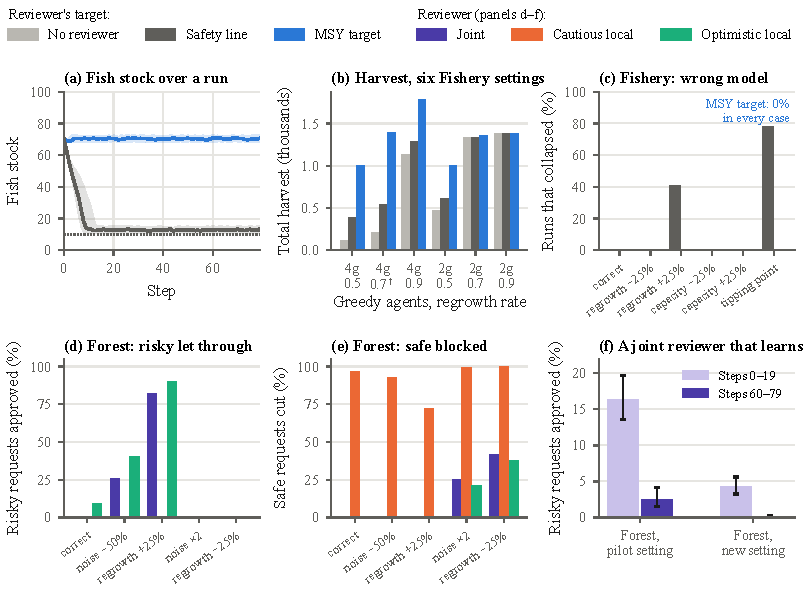
\includegraphics[width=\textwidth]{figures/fig2_reviewer.pdf}
  \caption{\textbf{What the reviewer aims for, and what it knows, decide how well it protects the resource.} Top row, \textsc{Fishery}: (a)~fish stock over one run when the reviewer sees all requests (4 greedy agents; line: middle run, band: 80\% of 64 populations). With only the safety line, the stock is fished down to just above 10; with the MSY target it stays near 70. (b)~Total harvest in six settings (``4g 0.7'' = 4 greedy agents, regrowth 0.7; $^\dagger$ the pilot setting). The MSY target gives more wherever the safety line limits anything (1,394 against 544 in the pilot setting). (c)~Share of runs in which the stock collapsed when the reviewer's model is wrong: 41\% (regrowth overestimated) and 78\% (an unknown tipping point) with the safety line, 0\% with the MSY target. Bottom row, \textsc{Forest}: (d)~risky requests let through and (e)~safe requests blocked, when one part of the reviewer's model is wrong. The direction of the error decides the mistake: thinking regrowth is faster lets 82\% of risky requests through; thinking it slower blocks 42\% of safe ones. The cautious local reviewer blocks most safe requests in every case. (f)~A joint reviewer that learns the model while running lets through 16\% of risky requests early and 2.5\% late. Error bars: 95\% intervals.}
  \label{fig:reviewer}
\end{figure}

\begin{figure}[H]
  \centering
  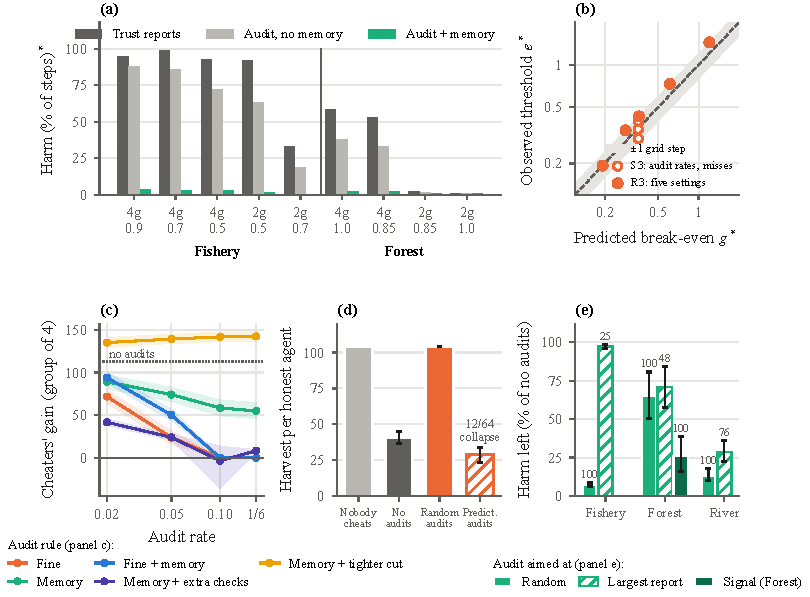
\includegraphics[width=\textwidth]{figures/fig3_audits.pdf}
  \caption{\textbf{What makes audits work: memory, an expected fine above the gain, and unpredictable targets.} (a)~Under-reporters in nine settings (one random audit per step, no fines). Auditing without memory barely reduces harm; remembering each caught lie removes most of it. $^*$\textsc{Fishery}: steps above the MSY limit; \textsc{Forest}: steps below the safety line. (b)~\textsc{Fishery}: each cheater's gain from cheating, on new runs, against the expected fine per step. Curves for audit rates from 1/6 to 0.02, and for audits that miss three cheats in four, fall on top of each other; every group stops between 0.30 and 0.40, near the break-even of 0.36. (c)~Cheaters' gain as the audit rate rises, under five audit rules (fine 6; bands: 95\% intervals). A fine stops cheating from an audit rate of 0.10. Memory alone leaves about half the gain. Tightening everyone's cut to allow for known cheaters makes cheating pay more than with no audits. (d)~Harvest per honest agent at the same audit rate (1/6) and fine (24): random audits stop cheating; predictable audits (every agent on every sixth step) leave honest agents worse off than no audits (28.8 against 40.9). (e)~\textsc{River} and an additive control, two under-reporters, one audit per step with memory: auditing the largest report gives more unsafe steps than auditing at random (3.4 points more in \textsc{River}, 95\% interval 1.8--5.3), because under-reporters keep their own reports small. Noticed after the run; experiment T1 tests it in all three games.}
  \label{fig:audits}
\end{figure}

\begin{table}[H]
  \centering\small
  \caption{\textbf{Audit rules compared} (\textsc{Fishery}, MSY target, 64 new populations). Cheaters' extra harvest: how much more the four cheaters get than if they complied, over 80 steps. Harvest per honest agent: what each honest agent gets. Checks per step include the extra checks that ``memory + extra checks'' spends watching known cheaters. Bold: best in column.}
  \label{tab:regimes}
  \resizebox{\textwidth}{!}{\begin{tabular}{llrrrr}
\toprule
Audit rule & Audit rate $q$ & Cheaters' extra harvest [95\% interval] & Harvest per honest agent & Steps over MSY limit (\%) & Checks per step \\
\midrule
No audits & --- & 112.8 [106, 120] & 39.5 & 100 & 0.00 \\
\addlinespace[2pt]
Fine & 0.10 & \textbf{0.0} & \textbf{104.1} & \textbf{0} & 0.61 \\
 & 1/6 & \textbf{0.0} & \textbf{104.1} & \textbf{0} & 1.00 \\
\addlinespace[2pt]
Lower allowance for caught agents & 0.10 & 58.4 [49, 68] & 74.5 & 54 & 0.61 \\
 & 1/6 & 55.1 [46, 65] & 77.1 & 49 & 1.00 \\
\addlinespace[2pt]
Check caught agents every round & 0.10 & $-$3.5 [$-$36, 14] & 95.2 & 16 & 3.78 \\
 & 1/6 & 8.3 [7, 10] & 99.4 & 10 & 4.07 \\
\addlinespace[2pt]
Lower allowance for all agents & 0.10 & 141.7 [136, 147] & 36.0 & 24 & 0.61 \\
 & 1/6 & 142.3 [137, 148] & 36.0 & 16 & 1.00 \\
\addlinespace[2pt]
Fine and lower allowance for all agents & 0.10 & \textbf{0.0} & \textbf{104.1} & \textbf{0} & 0.61 \\
 & 1/6 & \textbf{0.0} & \textbf{104.1} & \textbf{0} & 1.00 \\
\midrule
Nobody cheats & --- & 0 & 104.1 & 0 & 0 \\
\bottomrule
\end{tabular}
}
\end{table}
